\documentclass{article}

\pdfoutput=1
% AMS packages:
\usepackage[utf8x]{inputenc}
\usepackage{amsmath, amsthm, amsfonts }
\newcommand{\notimplies}{%
  \mathrel{{\ooalign{\hidewidth$\not\phantom{=}$\hidewidth\cr$\implies$}}}}
\usepackage{fullpage}
\usepackage{oz}
\usepackage[top = 2cm, bottom =2cm]{geometry}
\usepackage[hyperfootnotes=false]{hyperref}
\usepackage{url}
\usepackage{graphicx}
\usepackage{float}


\renewcommand{\figurename}{Figura}

% Shortcuts.
% One can define new commands to shorten frequently used
% constructions. As an example, this defines the R and Z used
% for the real and integer numbers.
%-----------------------------------------------------------------
\def\RR{\mathbb{R}}
\def\ZZ{\mathbb{Z}}

\title{ \bf   Projeto 04: Transmissão em redes}
\author{Hilário Fernandes de Araújo Júnior (92415)\\
Fernando Bandeira Soares (86281)
}


\begin{document}
\maketitle


\section{Objetivo}
O objetivo deste projeto é modelar uma rede de indivíduos em NetLogo e estudar a transmissão de uma doença que não necessariamente apresenta sintomas de forma imediata, como o resfriado.

\section{Construção do modelo}
O sistema estudado possui 500 neurônios (que representam individuos de uma certa espécie) que possuem links entre si de acordo com as seguintes topologias:

\begin{itemize}
\item Regular
\item Aleatória
\item Livre de Escala
\item Modularizada
\end{itemize}

Além disso, cada indivíduo pode assumir três estados: 

\begin{itemize}
\item Saudável (associado à cor verde): é um estado atingido por indivíduos que estão contaminados e com sintomas, de acordo com uma probabilidade pré-definida (variável \textit{recovery-chance}).
\item Contaminado sem sintomas (associado à cor azul): é um estado atingido por indivíduos saudáveis, de acordo com a probabilidade $P(i)=\sum_{j \in N(i)} s(j)$, em que $N(i)$ é a vizinhança de $i$, $s(j) = 1$ se o indivíduo $j$ está contaminado e sem sintomas, $s(j)=factor$ (onde \textit{factor} é uma variável determinada pelo usuário, valendo $0$ ou $1$) se o indíviduo está contaminado com sintomas e $s(j)=0$ caso o indivíduo $j$ esteja saudável.
\item Contaminado com sintomas (associado à cor vermelha): é um estado atingido por indivíduos que estão contaminados e sem sintomas após no máximo \textit{symptoms-show-max-time} ticks, onde esta variável é determinada pelo usuário.
\end{itemize}.

Foi convencionado que cada tick equivale a um dia. Também consideramos que a variável \textit{recovery-chance} assume o valor $12.4 \%$, pressupondo que o tempo médio em que a gripe é curada é de 8 dias, e consideramos que a variável \textit{symptoms-show-max-time} assume o valor 3.


\section{Resultados}
\subsection{Consenso}
Pelo fato de que indivíduos contaminados e com sintomas possuem uma probabilidade constante de se tornarem saudáveis, o sistema não torna-se homogêneo.

\begin{figure}[H]
  \centerline{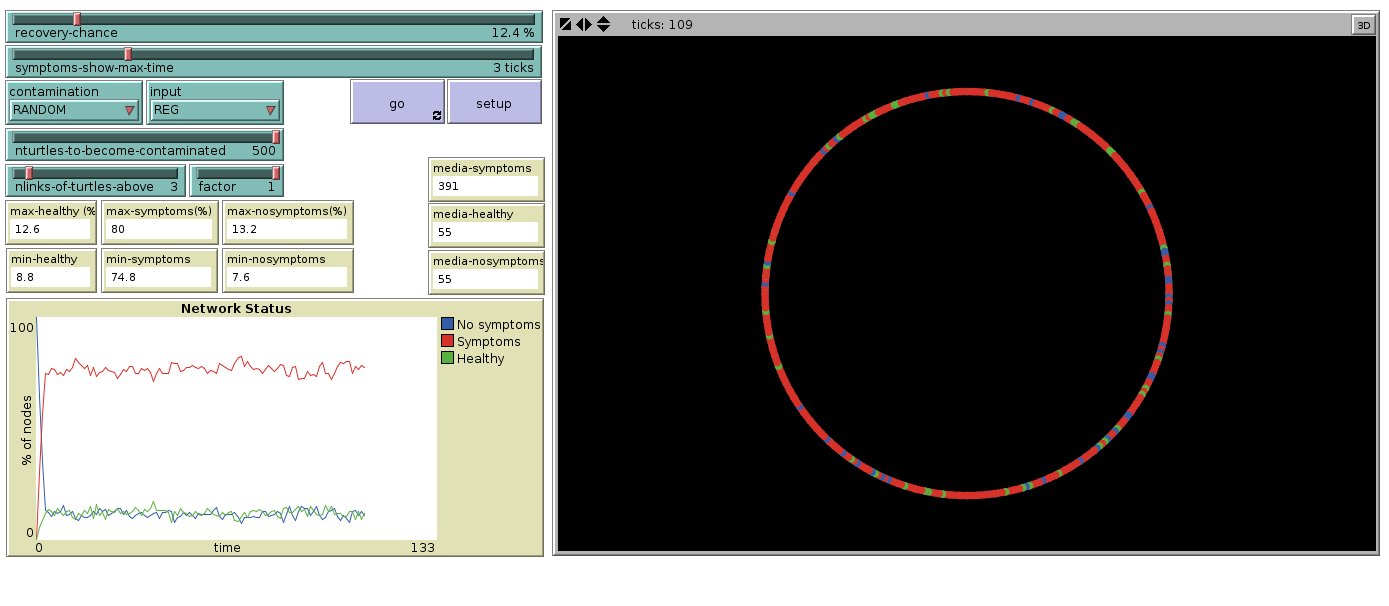
\includegraphics[width=\linewidth]{REG_consenso.png}}
  \caption{Valores de $x$ de 5 neurônios arbitrários na primeira Rede Regular.}
  \label{fig:boat1}
\end{figure}

\begin{figure}[H]
  \centerline{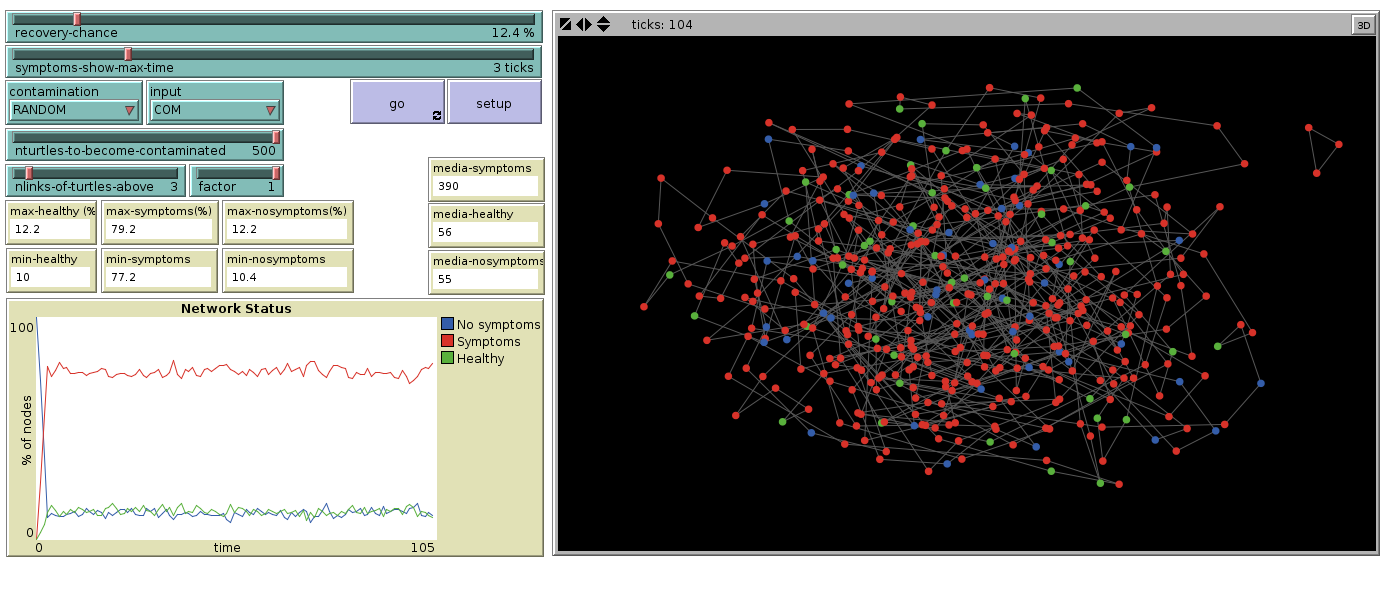
\includegraphics[width=\linewidth]{COM_consenso.png}}
  \caption{Valores de $x$ de 5 neurônios arbitrários na primeira Rede Regular.}
  \label{fig:boat1}
\end{figure}

\begin{figure}[H]
  \centerline{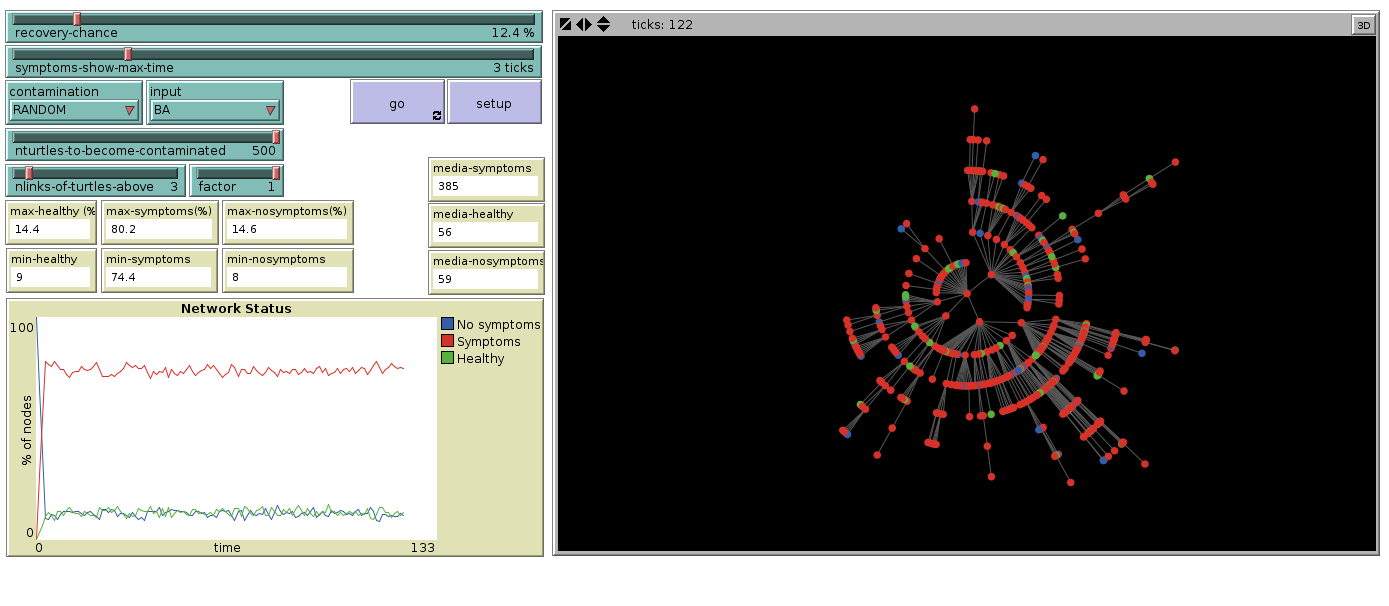
\includegraphics[width=\linewidth]{BA_consenso.png}}
  \caption{Valores de $x$ de 5 neurônios arbitrários na primeira Rede Regular.}
  \label{fig:boat1}
\end{figure}

\begin{figure}[H]
  \centerline{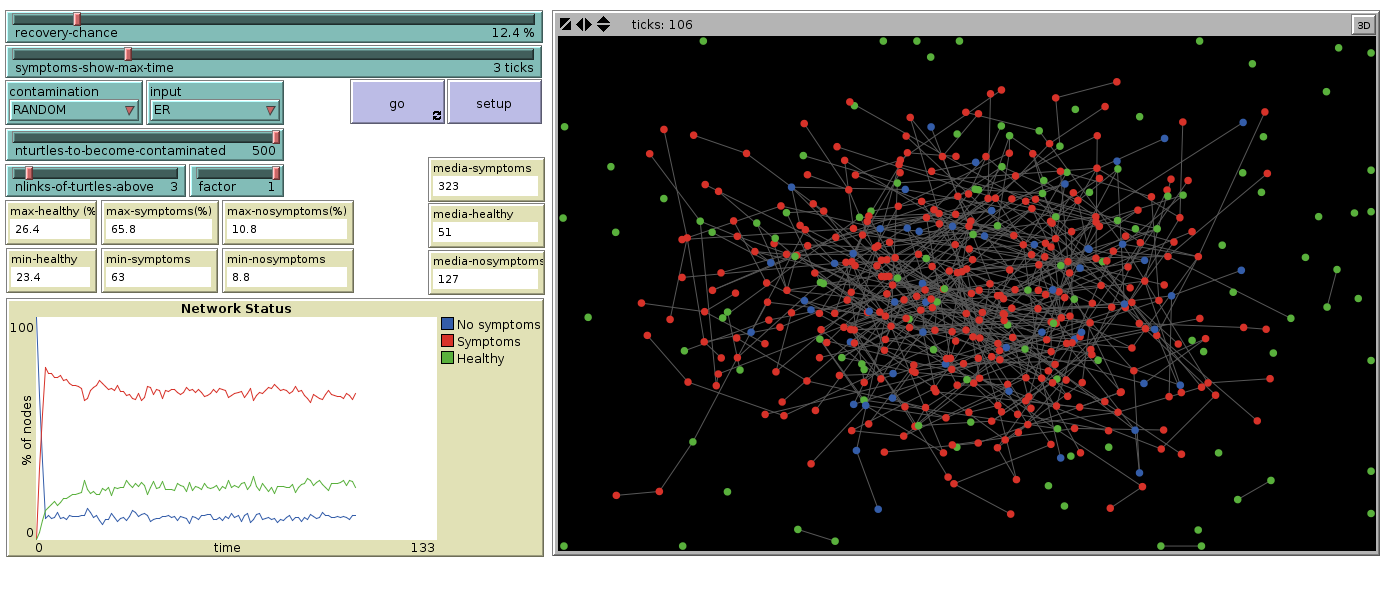
\includegraphics[width=\linewidth]{ER_consenso.png}}
  \caption{Valores de $x$ de 5 neurônios arbitrários na primeira Rede Regular.}
  \label{fig:boat1}
\end{figure}


\subsection{Tempo de Convergência}

\subsection{Número Inicial Mínimo de Contaminados Para o Espalhamento da Doença}

\subsection{Escolha dos Vértices}


%\begin{figure}[H]
  %\centerline{\includegraphics[width=\linewidth]{Grafico_REG.jpg}}
  %\caption{Valores de $x$ de 5 neurônios arbitrários na primeira Rede Regular.}
  %\label{fig:boat1}
%\end{figure}





\clearpage
 
\end{document}
